% GNUPLOT: LaTeX picture with Postscript
\begingroup
  \makeatletter
  \providecommand\color[2][]{%
    \GenericError{(gnuplot) \space\space\space\@spaces}{%
      Package color not loaded in conjunction with
      terminal option `colourtext'%
    }{See the gnuplot documentation for explanation.%
    }{Either use 'blacktext' in gnuplot or load the package
      color.sty in LaTeX.}%
    \renewcommand\color[2][]{}%
  }%
  \providecommand\includegraphics[2][]{%
    \GenericError{(gnuplot) \space\space\space\@spaces}{%
      Package graphicx or graphics not loaded%
    }{See the gnuplot documentation for explanation.%
    }{The gnuplot epslatex terminal needs graphicx.sty or graphics.sty.}%
    \renewcommand\includegraphics[2][]{}%
  }%
  \providecommand\rotatebox[2]{#2}%
  \@ifundefined{ifGPcolor}{%
    \newif\ifGPcolor
    \GPcolortrue
  }{}%
  \@ifundefined{ifGPblacktext}{%
    \newif\ifGPblacktext
    \GPblacktexttrue
  }{}%
  % define a \g@addto@macro without @ in the name:
  \let\gplgaddtomacro\g@addto@macro
  % define empty templates for all commands taking text:
  \gdef\gplbacktext{}%
  \gdef\gplfronttext{}%
  \makeatother
  \ifGPblacktext
    % no textcolor at all
    \def\colorrgb#1{}%
    \def\colorgray#1{}%
  \else
    % gray or color?
    \ifGPcolor
      \def\colorrgb#1{\color[rgb]{#1}}%
      \def\colorgray#1{\color[gray]{#1}}%
      \expandafter\def\csname LTw\endcsname{\color{white}}%
      \expandafter\def\csname LTb\endcsname{\color{black}}%
      \expandafter\def\csname LTa\endcsname{\color{black}}%
      \expandafter\def\csname LT0\endcsname{\color[rgb]{1,0,0}}%
      \expandafter\def\csname LT1\endcsname{\color[rgb]{0,1,0}}%
      \expandafter\def\csname LT2\endcsname{\color[rgb]{0,0,1}}%
      \expandafter\def\csname LT3\endcsname{\color[rgb]{1,0,1}}%
      \expandafter\def\csname LT4\endcsname{\color[rgb]{0,1,1}}%
      \expandafter\def\csname LT5\endcsname{\color[rgb]{1,1,0}}%
      \expandafter\def\csname LT6\endcsname{\color[rgb]{0,0,0}}%
      \expandafter\def\csname LT7\endcsname{\color[rgb]{1,0.3,0}}%
      \expandafter\def\csname LT8\endcsname{\color[rgb]{0.5,0.5,0.5}}%
    \else
      % gray
      \def\colorrgb#1{\color{black}}%
      \def\colorgray#1{\color[gray]{#1}}%
      \expandafter\def\csname LTw\endcsname{\color{white}}%
      \expandafter\def\csname LTb\endcsname{\color{black}}%
      \expandafter\def\csname LTa\endcsname{\color{black}}%
      \expandafter\def\csname LT0\endcsname{\color{black}}%
      \expandafter\def\csname LT1\endcsname{\color{black}}%
      \expandafter\def\csname LT2\endcsname{\color{black}}%
      \expandafter\def\csname LT3\endcsname{\color{black}}%
      \expandafter\def\csname LT4\endcsname{\color{black}}%
      \expandafter\def\csname LT5\endcsname{\color{black}}%
      \expandafter\def\csname LT6\endcsname{\color{black}}%
      \expandafter\def\csname LT7\endcsname{\color{black}}%
      \expandafter\def\csname LT8\endcsname{\color{black}}%
    \fi
  \fi
    \setlength{\unitlength}{0.0500bp}%
    \ifx\gptboxheight\undefined%
      \newlength{\gptboxheight}%
      \newlength{\gptboxwidth}%
      \newsavebox{\gptboxtext}%
    \fi%
    \setlength{\fboxrule}{0.5pt}%
    \setlength{\fboxsep}{1pt}%
\begin{picture}(8640.00,6480.00)%
    \gplgaddtomacro\gplbacktext{%
    }%
    \gplgaddtomacro\gplfronttext{%
      \csname LTb\endcsname%
      \put(176,4119){\rotatebox{-270}{\makebox(0,0){\strut{}$L$ ($L_\odot$)}}}%
      \put(4726,1474){\makebox(0,0){\strut{}$T$ (K)}}%
      \csname LTb\endcsname%
      \put(3871,1273){\makebox(0,0)[r]{\strut{}MESA star}}%
      \csname LTb\endcsname%
      \put(3871,1053){\makebox(0,0)[r]{\strut{}MESA star}}%
      \csname LTb\endcsname%
      \put(3871,833){\makebox(0,0)[r]{\strut{}MESA star}}%
      \csname LTb\endcsname%
      \put(3871,613){\makebox(0,0)[r]{\strut{}MESA star}}%
      \csname LTb\endcsname%
      \put(3871,393){\makebox(0,0)[r]{\strut{}MESA star}}%
      \csname LTb\endcsname%
      \put(3871,173){\makebox(0,0)[r]{\strut{}MESA star}}%
      \csname LTb\endcsname%
      \put(6706,1273){\makebox(0,0)[r]{\strut{}MESA star}}%
      \csname LTb\endcsname%
      \put(6706,1053){\makebox(0,0)[r]{\strut{}MESA star}}%
      \csname LTb\endcsname%
      \put(6706,833){\makebox(0,0)[r]{\strut{}MESA star}}%
      \csname LTb\endcsname%
      \put(6706,613){\makebox(0,0)[r]{\strut{}MESA star}}%
      \csname LTb\endcsname%
      \put(6706,393){\makebox(0,0)[r]{\strut{}Real Stars}}%
      \csname LTb\endcsname%
      \put(6706,173){\makebox(0,0)[r]{\strut{}Simulated Stars}}%
      \csname LTb\endcsname%
      \put(1078,2024){\makebox(0,0)[r]{\strut{}$10^{-12}$}}%
      \csname LTb\endcsname%
      \put(1078,2443){\makebox(0,0)[r]{\strut{}$10^{-10}$}}%
      \csname LTb\endcsname%
      \put(1078,2862){\makebox(0,0)[r]{\strut{}$10^{-8}$}}%
      \csname LTb\endcsname%
      \put(1078,3281){\makebox(0,0)[r]{\strut{}$10^{-6}$}}%
      \csname LTb\endcsname%
      \put(1078,3700){\makebox(0,0)[r]{\strut{}$10^{-4}$}}%
      \csname LTb\endcsname%
      \put(1078,4120){\makebox(0,0)[r]{\strut{}$10^{-2}$}}%
      \csname LTb\endcsname%
      \put(1078,4539){\makebox(0,0)[r]{\strut{}$10^{0}$}}%
      \csname LTb\endcsname%
      \put(1078,4958){\makebox(0,0)[r]{\strut{}$10^{2}$}}%
      \csname LTb\endcsname%
      \put(1078,5377){\makebox(0,0)[r]{\strut{}$10^{4}$}}%
      \csname LTb\endcsname%
      \put(1078,5796){\makebox(0,0)[r]{\strut{}$10^{6}$}}%
      \csname LTb\endcsname%
      \put(1078,6215){\makebox(0,0)[r]{\strut{}$10^{8}$}}%
      \csname LTb\endcsname%
      \put(8243,1804){\makebox(0,0){\strut{}$10^{3}$}}%
      \csname LTb\endcsname%
      \put(4727,1804){\makebox(0,0){\strut{}$10^{4}$}}%
      \csname LTb\endcsname%
      \put(1210,1804){\makebox(0,0){\strut{}$10^{5}$}}%
    }%
    \gplbacktext
    \put(0,0){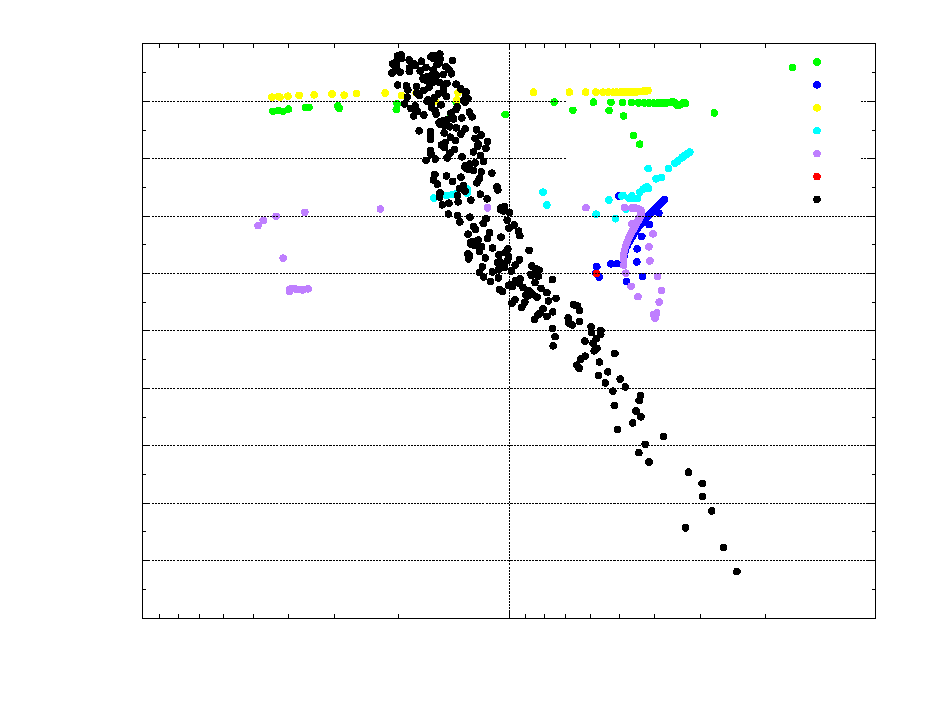
\includegraphics{./HR}}%
    \gplfronttext
  \end{picture}%
\endgroup
